%!TEX root = ../workbook-2014.tex

\section{Vector Mathematics in Python}

\numpy arrays support basic arithmetic operations that
correspond to the same operations on geometric vectors. The following examples illustrate this:
%
\begin{python}
>>> import numpy as npy
>>> x = np.array([1, 2, 3, 4, 5])
>>> y = np.array([6, 7, 8, 9, 10])
>>> x + y
array([ 7,  9, 11, 13, 15])
>>> x - y
array([-5, -5, -5, -5, -5])
>>> x * 3    # multiplication by a scalar
array([ 3,  6,  9, 12, 15])
>>> x * y    # elementwise multiplication of arrays, NOT dot product! 
array([ 6, 14, 24, 36, 50])
\end{python}
%
Above notice that the multiplication operator carries out element-wise multiplication.  The get the dot product we need to use the |dot()| function defined in \numpy.
%
\begin{python}
>>> np.dot(x, y)   # check your answer with pen and paper
130
\end{python}

In lecture we saw that many useful geometric properties of vectors could be expressed in the form of dot products. Let's start with some two-dimensional vectors where the geometry is  easy to visualize:

\begin{python}
>>> a = np.array((1, 0))
>>> b = np.array((0, 1))
\end{python}
%
Now let's draw our vectors:
%
\begin{python}
# create empty plot w/specified x- and y- limits
# set aspect ratio equal 
>>> ax = axes(aspect='equal')
>>> xlim(-1.5, 1.5)
>>> ylim(-1.5,1.5)
>>> ax.arrow(0, 0, a[0], a[1])
<matplotlib.patches.FancyArrow object at 0x108997450>
>>> ax.arrow(0, 0, b[0], b[1])
<matplotlib.patches.FancyArrow object at 0x10894bf10>
>>> show()
\end{python}
%
You should now have a figure that looks like the one below:
\begin{figure}[htbp]
\centering
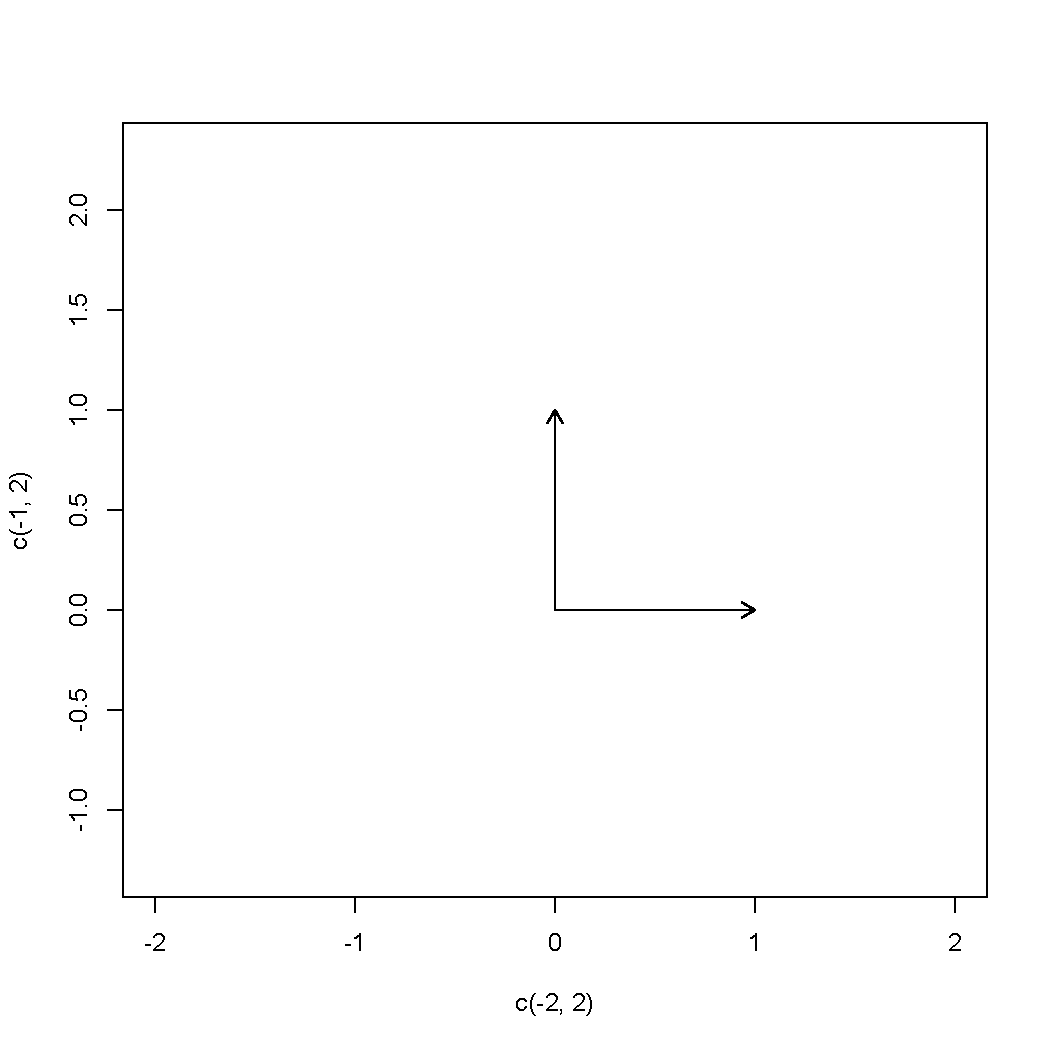
\includegraphics[width=0.33\columnwidth]{./figures/hands-on2/rightangle.pdf}
\caption{A simple vector figure.}
\end{figure}
%
Let's see what the dot product can tell us about these vectors. First recall that we can calculate the length of a vector as the square-root of the dot product of the vector with itself ($\vert\vec{a}\vert^2  =  \vec{a} \cdot \vec{a}$)
%
\begin{python}
>>> len_a = np.sqrt(np.dot(a, a))
>>> len_a
1.0
>>> len_b = np.sqrt(np.dot(b, b))
\end{python}
%
How about the angle between $a$ and $b$?
\begin{python}
>>> dot_ab = np.dot(a,b)
>>> dot_ab
0.0
>>> cos_ab = dot_ab / (len_a * len_b)
>>> cos_ab
0.0
\end{python}
A key point to remember dot product of two vectors is zero if, and only if, they are orthogonal to each other (regardless of their dimension).


